\documentclass[twoside]{article}

\usepackage{amsmath,amsthm,amssymb,graphicx}
\usepackage{hyperref}
\usepackage[numbers]{natbib}
\usepackage{float}
\usepackage{bbm}

\theoremstyle{definition}
\newtheorem{thm}{Theorem}[section]
\newtheorem{lem}[thm]{Lemma}
\newtheorem{prop}[thm]{Proposition}
\newtheorem{cor}[thm]{Corollary}
\newenvironment{pf}{{\noindent\sc Proof. }}{\qed}
\newenvironment{map}{\[\begin{array}{cccc}} {\end{array}\]}

\newcommand{\comment}[1]{}
\theoremstyle{definition}
\newtheorem*{defn}{Definition}
\newtheorem*{exmp}{Example}
\newtheorem*{prob}{Problem}

\theoremstyle{remark}
\newtheorem*{rem}{Remark}
\newtheorem*{note}{Note}
\newtheorem*{exer}{Exercise}

\setlength{\oddsidemargin}{0.25 in}
\setlength{\evensidemargin}{-0.25 in}
\setlength{\topmargin}{-0.6 in}
\setlength{\textwidth}{6.5 in}
\setlength{\textheight}{8.5 in}
\setlength{\headsep}{0.75 in}
\setlength{\parindent}{0 in}
\setlength{\parskip}{0.1 in}

\newcommand{\widgraph}[2]{\includegraphics[keepaspectratio,width=#1]{#2}}
\newcommand{\widgraphr}[3]{\includegraphics[keepaspectratio,width=#1,angle=#3]{#2}}

\newcommand{\lecture}[4]{
   \pagestyle{myheadings}
   \thispagestyle{plain}
   \newpage
   \setcounter{page}{1}
   \noindent
   \begin{center}
   \framebox{
      \vbox{\vspace{2mm}
    \hbox to 6.28in { {\bf Stat365/665 (Spring 2015) Data Mining and Machine Learning \hfill Lecture: #4} }
       \vspace{6mm}
       \hbox to 6.28in { {\Large \hfill #1  \hfill} }
       \vspace{6mm}
       \hbox to 6.28in { {\it Lecturer: #2 \hfill Scribe: #3} }
      \vspace{2mm}}
   }
   \end{center}
   \markboth{#1}{#1}
   \vspace*{4mm}
}


%%%%%%%
% Some commonly used notation
%%%%%%%

\def\R{{\mathbb R}}
\def\X{{\mathcal X}}
\def\Y{{\mathcal Y}}
\def\H{{\mathcal H}}
\def\E{{\mathbb E}}
\def\sign{{\rm sign}}

\newcommand{\percent}{$\%$}

\begin{document}
\textbf{Computer Vision, Homework 5}\\
\textbf{Leon Lixing Yu}\\

\section{Introduction}
The source code of the assignment is included in the package. The function file is $relaxed = relaximage(image, niters)$. The top level wrapper of the function (a.k.a. program entry) is $hw5.m$.\\
I have taken reference from $http://www.mathworks.com/matlabcentral/fileexchange/34807-nonlinear-relaxation-labeling-for-image-processing$. Since the reference has pretty good data struct, I used its data structure.\\
The following sections explains the questions of the assignment.\\
\section{What are the nodes?}
The nodes of relaxiation labelling is simply the pixels of each image. The neighbours of each node is the neighbouring pixels of the particular pixel. For example, if the particular pixel is $N0$, and the neighbouring pixels are $n1, n2, n3, n4, n5, n6, n7, n8$. Below are the illustration of the neighbourhood.
\[n1\;\;n2\;\;n3\]
\[n4\;\;N0\;\;n5\]
\[n6\;\;n7\;\;n8\]
As a result, each node has 8 neighbours, and the neighbourhood has 8 nodes. When the node is at the edge of the frame, I fill the unfilled slots with replicated confidences.\\
\section{What are the labels?}
Since this is a binary labelling problem, we will only have two labels, foreground (objects) and background. Background are white, and objects are black as shown in the given pictures. 
\section{What are the initial confidences be set?}
The initial confidences is the pixel density of each node. The pixel density ranges from $0$ to $255$ in the original image as 255 being all baclk and 0 being all white. To make it between 0 and 1, I divided all pixels by 255. \\
After division, the probabilty of the node being a part of the object, $P_{object}$ is $density/255$, and the probability of the node being a part of the background, $P_{background}$ is $1 - P_{object}$ for all pixels (nodes).

\section{What should the neighbourhood relationships be?}
For all 8 neighhours ($P_{neighbour}$) of the chosen node ($P_{node}$):\\

$\;\;\;\;$    compute $P(object|object)$, this notation stands for $P_{node}(object)\;\; given\;\; P_{neighbour}(object)$\\

$\;\;\;\;$     do the same thing for $P(object|background)$, $P(background|background)$, and $P(background|object)$. \\

$\;\;\;\;$     This step can be interrupted as what is current node's probability of being object or background if the given neighbour has $x$ probablity of being background or object.\\
    
$\;\;\;\;$     and then divide the results by $(P_{node}(object))$\\
    
$\;\;\;\;$     This is our results for neighbourhood relationships. \\

\section{How should the compatibility fields be structured?}
For each labels (we only have 2)\\
    The compatibility is the sum of $P_{neighbour} * neighbourhood\;relationhips$ for all neighbours.

\section{results}

\begin{figure}[H]
\centering
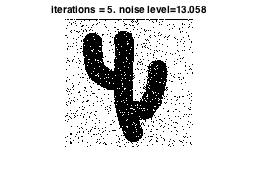
\includegraphics[width=60mm]{5_cactus.jpg}
\caption{cactus picture with 5 iterations, we see there are a lot of noises}
\end{figure}

\begin{figure}[H]
\centering
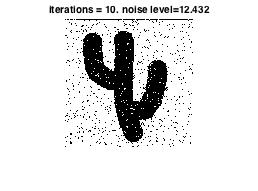
\includegraphics[width=60mm]{10_cactus.jpg}
\caption{cactus picture with 10 iterations, noise reduces}
\end{figure}

\begin{figure}[H]
\centering
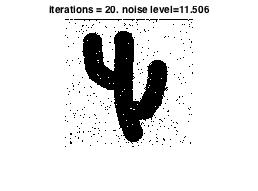
\includegraphics[width=60mm]{20_cactus.jpg}
\caption{cactus picture with 20 iterations, noise reduces}
\end{figure}

\begin{figure}[H]
\centering
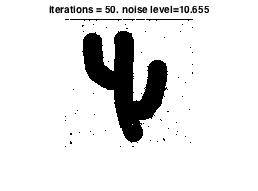
\includegraphics[width=60mm]{50_cactus.jpg}
\caption{cactus picture with 50 iterations, noise reduces}
\end{figure}

\begin{figure}[H]
\centering
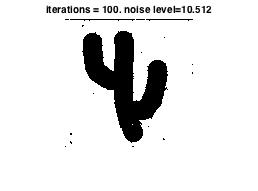
\includegraphics[width=60mm]{100_cactus.jpg}
\caption{cactus picture with 100 iterations, noise reduces slightly}
\end{figure}

\begin{figure}[H]
\centering
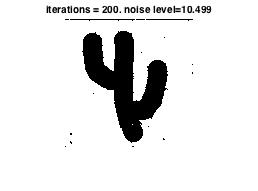
\includegraphics[width=60mm]{200_cactus.jpg}
\caption{cactus picture with 100 iterations, we can barely see any improvement. Since the algorithm does not gauarntee converge, it is possible that relaxiation labelling reaches a limit}
\end{figure}

\begin{figure}[H]
\centering
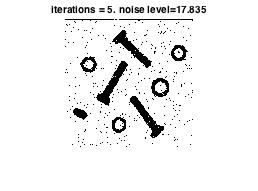
\includegraphics[width=60mm]{5_parts.jpg}
\caption{ parts picture with 5 iterations, we see there are a lot of noises}
\end{figure}

\begin{figure}[H]
\centering
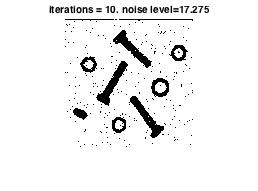
\includegraphics[width=60mm]{10_parts.jpg}
\caption{parts picture with 10 iterations, noise reduces}
\end{figure}

\begin{figure}[H]
\centering
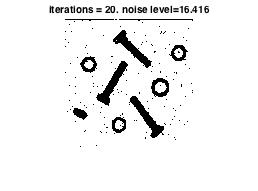
\includegraphics[width=60mm]{20_parts.jpg}
\caption{parts  picture with 20 iterations, noise reduces}
\end{figure}

\begin{figure}[H]
\centering
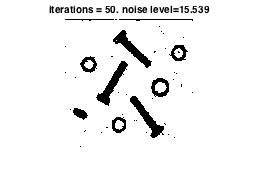
\includegraphics[width=60mm]{50_parts.jpg}
\caption{parts  picture with 50 iterations, noise reduces}
\end{figure}

\begin{figure}[H]
\centering
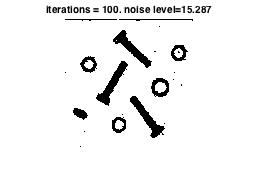
\includegraphics[width=60mm]{100_parts.jpg}
\caption{parts  picture with 100 iterations, noise reduces slightly}
\end{figure}

\begin{figure}[H]
\centering
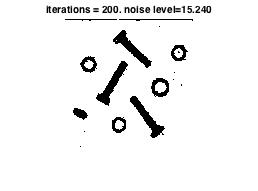
\includegraphics[width=60mm]{200_parts.jpg}
\caption{parts  picture with 200 iterations, we can barely see any improvement. Since the algorithm does not gauarntee converge, it is possible that relaxiation labelling reaches a limit. However, I do see nosie level reduces}
\end{figure}

\begin{figure}[H]
\centering
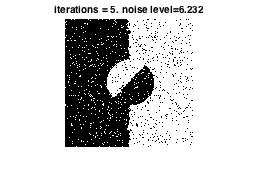
\includegraphics[width=60mm]{5_bump.jpg}
\caption{bump picture with 5 iterations, we see that instead of showing a bump-ish figure, it shows a black-white sphere, which is not really what we are looking for, the main reason is that the bump picture has the shading effect, and our probability model only makes a binary decision (black $\rightarrow$ object, white $\rightarrow$ background), meaning if P is less than 0.5 it is considered background, vise versa. }
\end{figure}

\begin{figure}[H]
\centering
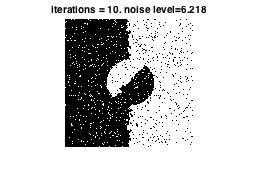
\includegraphics[width=60mm]{10_bump.jpg}
\caption{bump picture with 10 iterations, noise reduces, but it still only shows binary decisions}
\end{figure}

\begin{figure}[H]
\centering
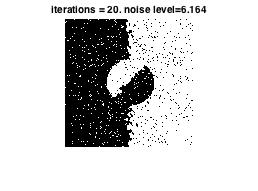
\includegraphics[width=60mm]{20_bump.jpg}
\caption{bump picture with 20 iterations, noise reduces}
\end{figure}

\begin{figure}[H]
\centering
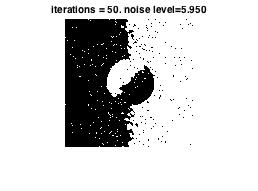
\includegraphics[width=60mm]{50_bump.jpg}
\caption{bump picture with 50 iterations, noise reduces}
\end{figure}

\begin{figure}[H]
\centering
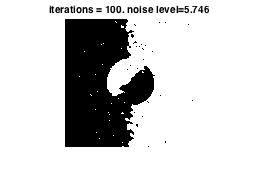
\includegraphics[width=60mm]{100_bump.jpg}
\caption{bump picture with 100 iterations, noise reduces slightly}
\end{figure}

\begin{figure}[H]
\centering
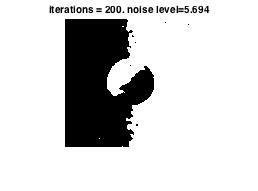
\includegraphics[width=60mm]{200_bump.jpg}
\caption{bump picture with 200 iterations. Though the noises are removed, we see some unwanted shapes, and I have explained the reasons in iteration=5 picture. }
\end{figure}

\end{document}
